\chapter{Fully homomorphic encryption: Introduction and
bootstrapping}\label{chapfheone}

In today's era of ``cloud computing'', much of individuals' and
businesses' data is stored and computed on by third parties such as
Google, Microsoft, Apple, Amazon, Facebook, Dropbox and many others.
Classically, cryptography provided solutions to protecting
\href{https://www.schneier.com/blog/archives/2010/06/data_at_rest_vs.html}{data
in motion} from point A to point B. But these are not always sufficient
to protect \href{https://en.wikipedia.org/wiki/Data_at_rest}{data at
rest} and particularly
\href{https://en.wikipedia.org/wiki/Data_in_use}{data in use}. For
example, suppose that \emph{Alice} has some data \(x \in \{0,1\}^n\) (in
modern applications \(x\) would well be terabytes in length or larger)
that she wishes to store with the cloud service \emph{Bob}, but is
afraid that Bob will be hacked, subpoenaed or simply does not completely
trust Bob.

Encryption does not seem to immediately solve the problem. Alice could
store at Bob an \emph{encrypted} version of the data and keep the secret
key for herself. But then she would be at a loss if she wanted to do
with the data anything more than retrieving particular blocks of it. If
she wanted to outsource computation to Bob as well, and compute \(f(x)\)
for some function \(f\), then she would need to share the secret key
with Bob, thus defeating the purpose of encrypting the data in the first
place.

For example, after the computing systems of Office of Personell
Management (OPM) were
\href{https://www.lawfareblog.com/why-opm-hack-far-worse-you-imagine}{discovered
to be hacked} in June of 2015, revealing sensitive information,
including fingerprints and all data gathered during security clearance
checks of up to 18 million people, DHS assistant secretary for
cybersecurity and communications Andy Ozment
\href{http://www.federaltimes.com/story/government/omr/opm-cyber-report/2015/06/19/opm-breach-encryption/28985237/}{said}
that encryption wouldn't have helped preventing it since ``if an
adversary has the credentials of a user on the network, then they can
access data even if it's encrypted, just as the users on the network
have to access data''. So, can we encrypt data in a way that still
allows some access and computing on it?

Already in 1978,
\href{http://luca-giuzzi.unibs.it/corsi/Support/papers-cryptography/RAD78.pdf}{Rivest,
Adleman and Dertouzos} considered this problem of a business that wishes
to use a ``commercial
\href{https://en.wikipedia.org/wiki/Time-sharing}{time-sharing}
service'' to store some sensitive data. They envisioned a potential
solution for this task which they called a privacy homomorphism. This
notion later became known as \emph{fully homomorphic encryption (FHE)}
which is an encryption that allows a party (such as the cloud provider)
that \emph{does not know the secret key} to modify a ciphertext \(c\)
encrypting \(x\) to a ciphertext \(c'\) encrypting \(f(x)\) for every
efficiently computable \(f()\). In particular in our scenario above (see
\cref{fhefig}), such a scheme will allow Bob, given an encryption of
\(x\), to compute the encryption of \(f(x)\) and send this ciphertext to
Alice without ever getting the secret key and so without ever learning
anything about \(x\) (or \(f(x)\) for that matter).

\begin{marginfigure}
\centering
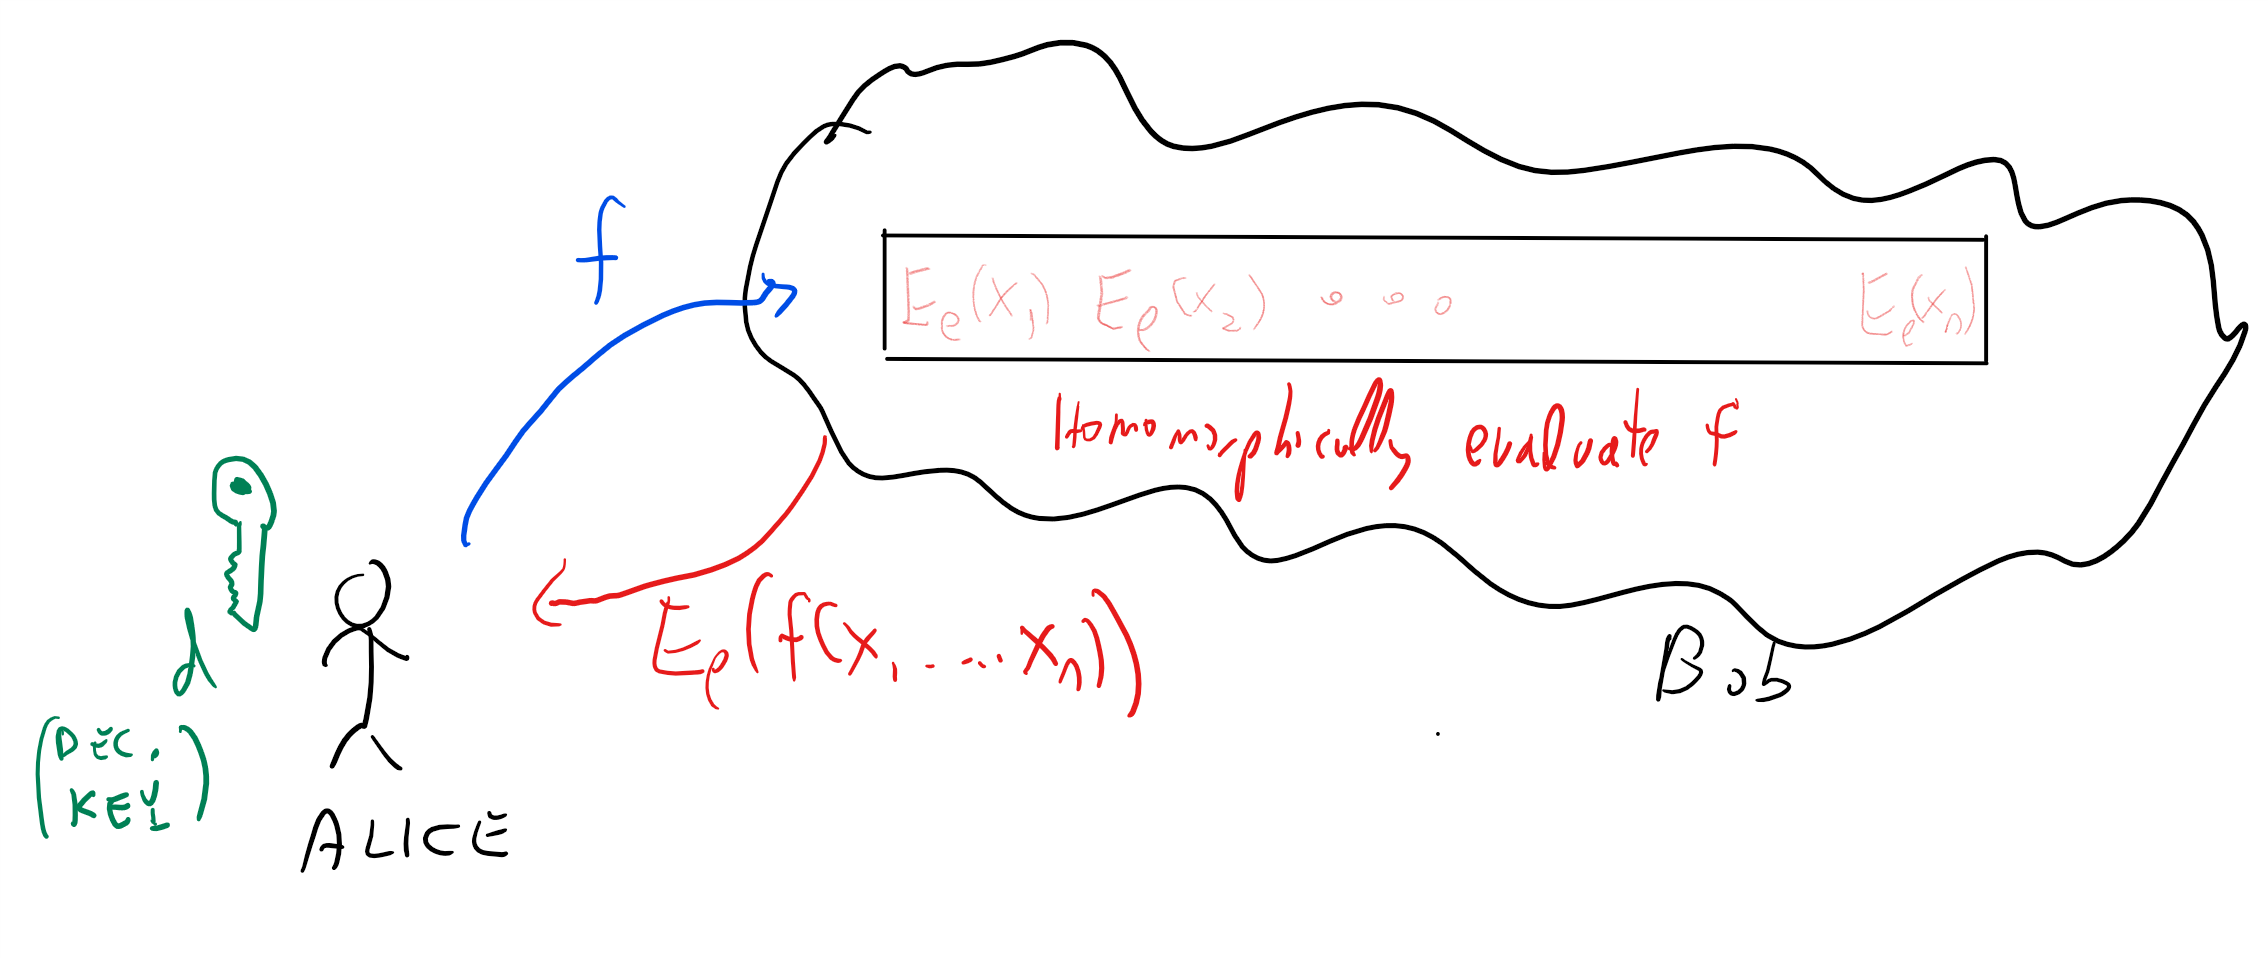
\includegraphics[width=\linewidth, height=1.5in, keepaspectratio]{../figure/fhedescription.png}
\caption{A fully homomorphic encryption can be used to store data on the
cloud in encrypted form, but still have the cloud provider be able to
evaluate functions on the data in encrypted form (without ever learning
either the inputs or the outputs of the function they evaluate).}
\label{fhefig}
\end{marginfigure}

Unlike the case of a trapdoor function, where it only took a year for
Diffie and Hellman's challenge to be answered by RSA, in the case of
fully homomorphic encryption for more than 30 years cryptographers had
no constructions achieving this goal. In fact, some people suspected
that there is something inherently incompatible between the security of
an encryption scheme and the ability of a user to perform all these
operations on ciphertexts. Stanford cryptographer Dan Boneh used to joke
to incoming graduate students that he will immediately sign the thesis
of anyone who came up with a fully homomorphic encryption. But he never
expected that he will actually encounter such a thesis, until in 2009,
Boneh's student Craig Gentry released a
\href{https://crypto.stanford.edu/craig/}{paper} doing just that.
Gentry's paper shook the world of cryptography, and instigated a flurry
of research results making his scheme more efficient, reducing the
assumptions it relied on, extending and applying it, and much more. In
particular, Brakerski and Vaikuntanathan managed to obtain a fully
homomorphic encryption scheme based only on the \emph{Learning with
Error (LWE)} assumption we have seen before.

Although there is an \href{http://shaih.github.io/HElib/}{open source
library}, as well as
\href{https://www.dcsec.uni-hannover.de/fileadmin/ful/mitarbeiter/brenner/wahc14_RC.pdf}{other}
\href{https://eprint.iacr.org/2014/816}{implementations}, there is still
much work to be done in order to turn FHE from theory to practice. For a
comparable level of security, the encryption and decryption operations
of a fully homomorphic encryption scheme are several orders of magnitude
slower than a conventional public key system, and (depending on its
complexity) homomorphically evaluating a circuit can be significantly
more taxing. However, this is a fast evolving field, and already since
2009 significant optimizations have been discovered that reduced the
computational and storage overhead by many orders of magnitudes. As in
public key encryption, one would imagine that for larger data one would
use a ``hybrid'' approach of combining FHE with symmetric encryption,
though one might need to come up with tailor-made symmetric encryption
schemes that can be efficiently evaluated.\footnote{In
  \href{https://eprint.iacr.org/2012/099.pdf}{2012} the state of art on
  homomorphically evaluating AES was about six orders of magnitude
  slower than non-homomorphic AES computation. I don't know what's the
  current record.}

In this lecture and the next one we will focus on the fully homomorphic
encryption schemes that are \emph{easiest to describe}, rather than the
ones that are most \emph{efficient} (though the efficient schemes share
many similarities with the ones we will talk about). As is generally the
case for lattice based encryption, the current most efficient schemes
are based on \emph{ideal} lattices and on assumptions such as ring LWE
or the security of the NTRU cryptosystem.\footnote{As we mentioned
  before, as a general rule of thumb, the difference between the ideal
  schemes and the one that we describe is that in the ideal setting one
  deals with \emph{structured} matrices that have a compact
  representation as a single vector and also enable fast FFT-like
  matrix-vector multiplication. This saves a factor of about \(n\) in
  the storage and computation requirements (where \(n\) is the dimension
  of the subspace/lattice). However, there can be some subtle security
  implications for ideal lattices as well, see e.g.,
  \href{https://eprint.iacr.org/2016/127}{here},
  \href{https://eprint.iacr.org/2015/313}{here},
  \href{https://eprint.iacr.org/2016/139}{here}, and
  \href{https://eprint.iacr.org/2015/676}{here}.}

\hypertarget{verifyinglessonrem}{}
\begin{remark}[Lesson from verifying computation] \label[remark]{verifyinglessonrem}

To take the distance between theory and practice in perspective, it
might be useful to consider the case of \emph{verifying computation}. In
the early 1990's researchers (motivated initially by zero knowledge
proofs) came up with the notion of
\href{http://madhu.seas.harvard.edu/papers/2009/pcpcacm.pdf}{probabilistically
checkable proofs (PCP's)} which could yield in principle extremely
succinct ways to check correctness of computation.

Probabilistically checkable proofs can be thought of as ``souped up''
versions of NP completeness reductions and like these reductions, have
been mostly used for \emph{negative} results, especially since the
initial proofs were extremely complicated and also included enormous
hidden constants. However, with time people have slowly understood these
better and made them more efficient (e.g., see
\href{http://m.cacm.acm.org/magazines/2015/2/182636-verifying-computations-without-reexecuting-them/fulltext}{this
survey}) and it has now reached the point where these results, are
\href{http://cacm.acm.org/magazines/2016/2/197429-pinocchio/abstract}{nearly
practical} (see also \href{https://eprint.iacr.org/2016/646}{this}) and
in fact these ideas underly at least one \href{http://z.cash}{startup}.
Overall, constructions for verifying computation have improved by at
least 20 orders of magnitude over the last two decades. (We will talk
about some of these constructions later in this course.) If progress on
fully homomorphic encryption follows a similar trajectory, then we can
expect the road to practical utility to be very long, but there is hope
that it's not a ``bridge to nowhere''.

\end{remark}

\hypertarget{hardwarefhe}{}
\begin{remark}[Poor man's FHE via hardware] \label[remark]{hardwarefhe}

Since large scale fully homomorphic encryption is still impractical,
people have been trying to achieve at least weaker security goals using
certain assumptions. In particular Intel chips have so called
\href{https://goo.gl/HW4pPU}{``Secure enclaves''} which one can think of
as a somewhat tamper-protected region of the processor that is supposed
to be out of reach for the outside world. The idea is that a cloud
provider client would treat this enclave as a trusted party that it can
communicate with through the cloud provider. The client can store their
data on the cloud encrypted with some key \(k\), and then set up a
secure channel with the enclave using an authenticated key exchange
protocol, and send \(k\) over. Then, when the client sends over a
function \(f\) to the cloud provider, the latter party can simulate FHE
by asking the enclave to compute the encryption of \(f(x)\) given the
encryption of \(x\). In this solution ultimately the private key does
reside on the cloud provider's computers, and the client has to trust
the security of the enclave. In practice, this could provide reasonable
security against remote hackers, but (unlike FHE) probably not against
sophisticated attackers (e.g., governments) that have physical access to
the server.

\end{remark}

\section{Defining fully homomorphic
encryption}\label{16-Defining-fully-homomor}

We start by defining \emph{partially homomorphic} encryption. We focus
on encryption for single bits. This is without loss of generality for
CPA security (CCA security is anyway ruled out for homomorphic
encryption- can you see why?), though there are more efficient
constructions that encrypt several bits at a time.

\hypertarget{partialhomdef}{}
\begin{definition}[Partially Homomorphic Encryption] \label[definition]{partialhomdef}

Let \(\mathcal{F} = \cup \mathcal{F}_\ell\) be a class of functions
where every \(f\in\mathcal{F}_\ell\) maps \(\{0,1\}^\ell\) to
\(\{0,1\}\).\\
An \emph{\(\mathcal{F}\)-homomorphic public key encryption scheme} is a
CPA secure public key encryption scheme \((G,E,D)\) such that there
exists a polynomial-time algorithm
\(\ensuremath{\mathit{EVAL}}:\{0,1\}^* \rightarrow \{0,1\}^*\) such that
for every \((e,d)=G(1^n)\), \(\ell=poly(n)\),
\(x_1,\ldots,x_\ell \in \{0,1\}\), and \(f\in \mathcal{F}_\ell\) of
description size \(|f|\) at most \(poly(\ell)\) it holds that:

\begin{itemize}
\item
  \(c=\ensuremath{\mathit{EVAL}}_e(f,E_e(x_1),\ldots,E_e(x_\ell))\) has
  length at most \(n\).
\item
  \(D_d(c)=f(x_1,\ldots,x_\ell)\).
\end{itemize}

\end{definition}

\begin{pause} \label[pause]{16-Please-stop-and-verify}

Please stop and verify you understand the definition. In particular you
should understand why some bound on the length of the output of
\(\ensuremath{\mathit{EVAL}}\) is needed to rule out trivial
constructions that are the analogous of the cloud provider sending over
to Alice the entire encrypted database every time she wants to evaluate
a function of it. By artificially increasing the randomness for the key
generation algorithm, this is equivalent to requiring that
\(|c| \leq p(n)\) for some fixed polynomial \(p(\cdot)\) that does not
grow with \(\ell\) or \(|f|\). You should also understand the
distinction between ciphertexts that are the output of the encryption
algorithm on the plaintext \(b\), and ciphertexts that decrypt to \(b\),
see \cref{evalciphertextfig}.

\end{pause}

\begin{marginfigure}
\centering
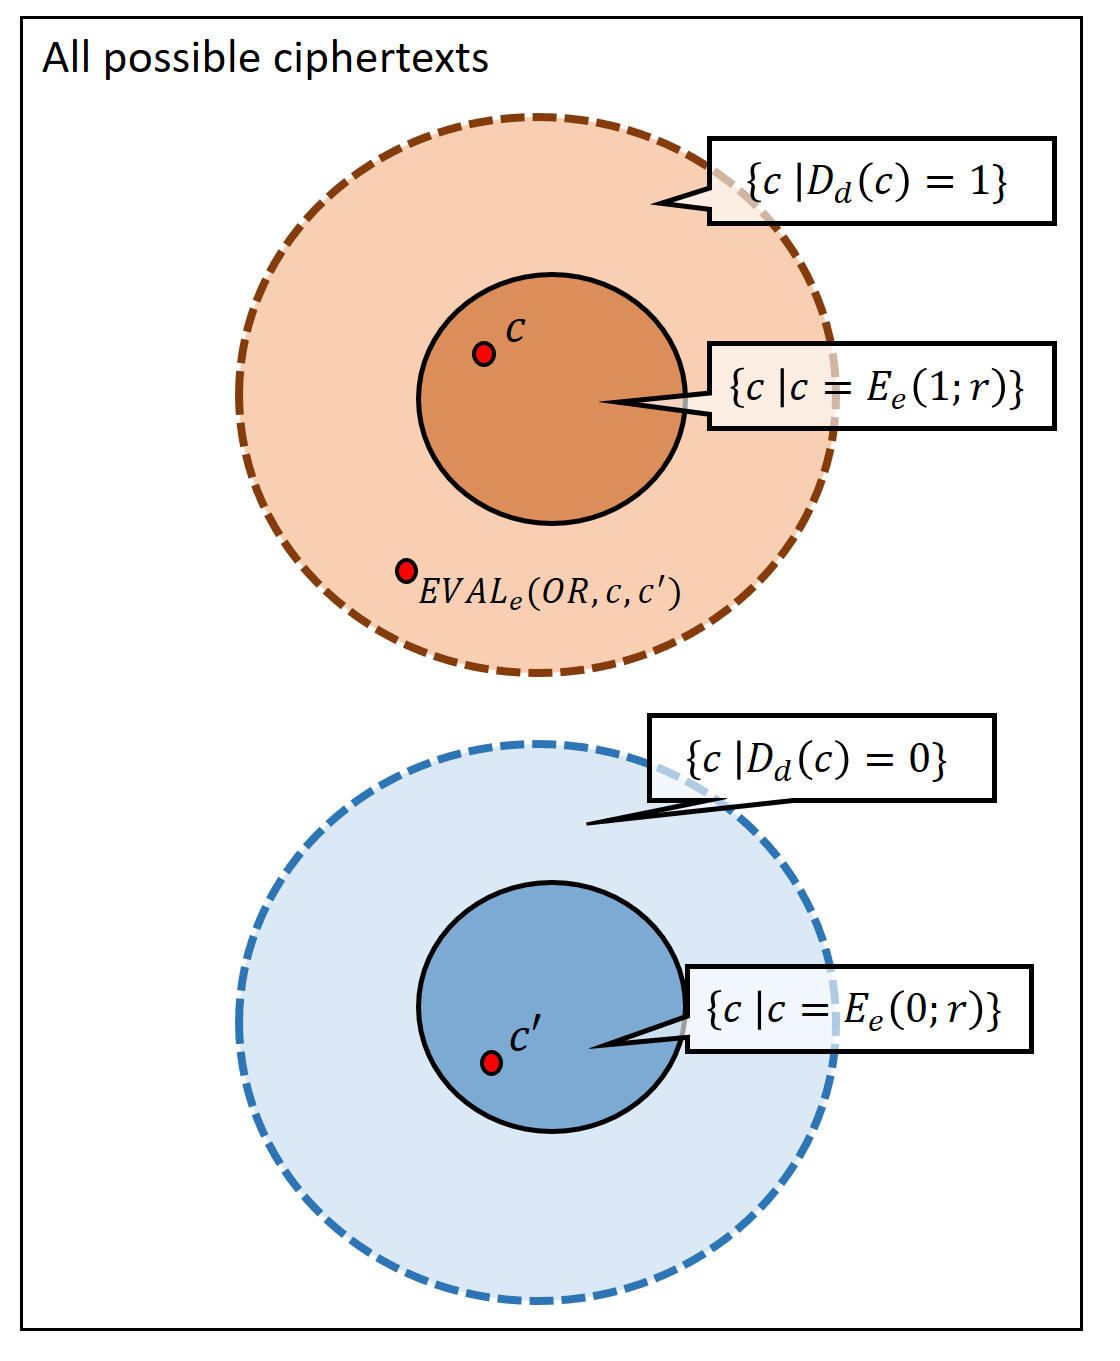
\includegraphics[width=\linewidth, height=1.5in, keepaspectratio]{../figure/evalciphertexts.png}
\caption{In a valid encryption scheme \(E\), the set of ciphertexts
\(c\) such that \(D_d(c)=b\) is a superset of the set of ciphertexts
\(c\) such that \(c=E_e(b;r)\) for some \(r \in \{0,1\}^{t}\) where
\(t\) is the number of random bits used by the encryption algorithm. Our
definition of partially homomorphic encryption scheme requires that for
every \(f:\{0,1\}^\ell \rightarrow \{0,1\}\) in our family and
\(x\in \{0,1\}^\ell\), if \(c_i \in E_e(x_i;\{0,1\}^t)\) for
\(i=1..\ell\) then \(\ensuremath{\mathit{EVAL}}(f,c_1,\ldots,c_\ell)\)
is in the superset \(\{ c \;|\; D_d(c)=f(x) \}\) of
\(E_e(f(x);\{0,1\}^t)\). For example if we apply
\(\ensuremath{\mathit{EVAL}}\) to the \(\ensuremath{\mathit{OR}}\)
function and ciphertexts \(c,c'\) that were obtained as encryptions of
\(1\) and \(0\) respectively, then the output is a ciphertext \(c''\)
that would be decrypted to \(\ensuremath{\mathit{OR}}(1,0)=1\), even if
\(c''\) is not in the smaller set of possible outputs of the encryption
algorithm on \(1\). This distinction between the smaller and larger set
is the reason why we cannot automatically apply the
\(\ensuremath{\mathit{EVAL}}\) function to ciphertexts that are obtained
from the outputs of previous \(\ensuremath{\mathit{EVAL}}\) operations.}
\label{evalciphertextfig}
\end{marginfigure}

A \emph{fully homomomorphic encryption} is simply a partially
homomorphic encryption scheme for the family \(\mathcal{F}\) of
\emph{all} functions, where the description of a function is as a
circuit (say composed of
\href{https://en.wikipedia.org/wiki/NAND_gate}{NAND} gates, which are
known to be a universal basis).

\subsection{Another application: fully homomorphic encryption for
verifying computation}\label{16-Another-application-fu}

The canonical application of fully homomorphic encryption is for a
client to store encrypted data \(E(x)\) on a server, send a function
\(f\) to the server, and get back the encryption \(E(f(x))\) of
\(f(x)\). This ensures that the server does not learn any information
about \(x\), but does not ensure that it actually computes the correct
function!

Here is a cute protocol to achieve the latter goal (due to
\href{https://eprint.iacr.org/2010/241}{Chung Kalai and Vadhan}).
Curiously the protocol involves ``doubly encrypting'' the input, and
homomorphically evaluating the \(\ensuremath{\mathit{EVAL}}\) function
itself.

\begin{itemize}
\item
  \textbf{Assumptions:} We assume that all functions \(f\) that the
  client will be interested in can be described by a string of length
  \(n\).
\item
  \textbf{Preprocessing:} The client generates a pair of keys \((e,d)\).
  In the initial stage the client computes the encrypted database
  \(\overline{c}=E_e(x)\) and sends \(\overline{c},e,e'\) to the server.
  It also computes \(c^* = E_e(f^*)\) for some function \(f^*\) as well
  as \(C^{**}=\ensuremath{\mathit{EVAL}}_{e}(eval,c^*\|\overline{c})\)
  for some function \(f^*\) and keeps \(c^*,c^{**}\) for herself, where
  \(eval(f,x)=f(x)\) is the circuit evaluation function.
\item
  \textbf{Client query:} To ask for an evaluation of \(f\), the client
  generates a new random FHE keypair \((e',d')\), chooses
  \(b \leftarrow_R \{0,1\}\) and lets \(c_b = E_{e'}(E_e(f))\) and
  \(c_{1-b}=E_{e'}(c^*)\). It sends the triple \(e',c_0,c_1\) to the
  server.
\item
  \textbf{Server response:} Given the queries \(c_0,c_1\), the server
  defines the function \(g:\{0,1\}^* \rightarrow \{0,1\}^*\) where
  \(g(c)=\ensuremath{\mathit{EVAL}}_e(eval,c\|\overline{c})\) (for the
  fixed \(\overline{c}\) received) and computes \(c'_0,c'_1\) where
  \(c'_b = \ensuremath{\mathit{EVAL}}_{e'}(g_b,c_b)\). (Please pause
  here and make sure you understand what this step is doing! Note that
  we use here crucially the fact that \(\ensuremath{\mathit{EVAL}}\)
  itself is a polynomial time computation.)
\item
  \textbf{Client check:} Client checks whether
  \(D_{d'}(c'_{1-b})=c^{**}\) and if so accepts \(D_d(D_{d'}(c'_b))\) as
  the answer.
\end{itemize}

We claim that if the server cheats then the client will detect this with
probability \(1/2 - negl(n)\). Working this out is a great exercise. The
probability of detection can be amplified to \(1-negl(n)\) using
appropriate repetition, see the paper for details.

\section{Example: An XOR homomorphic
encryption}\label{16-Example-An-XOR-homomor}

It turns out that Regev's LWE-based encryption LWEENC we saw before is
homomorphic with respect to the class of linear (mod 2) functions. Let
us recall the LWE assumption and the encryption scheme based on it.

\hypertarget{LWEdef}{}
\begin{definition}[LWE (simplified decision variant)] \label[definition]{LWEdef}

Let \(q=q(n)\) be some function mapping the natural numbers to primes.
The \emph{\(q(n)\)-decision learning with error (\(q(n)\)-dLWE)
conjecture} is the following: for every \(m=poly(n)\) there is a
distribution \(\ensuremath{\mathit{LWE}}_q\) over pairs \((A,s)\) such
that:

\begin{itemize}
\item
  \(A\) is an \(m\times n\) matrix over \(\Z_q\) and \(s\in\Z_q^n\)
  satisfies \(s_1=\floor{\tfrac{q}{2}}\) and \(|As|_i \leq \sqrt{q}\)
  for every \(i\in \{1,\ldots, m\}\).
\item
  The distribution \(A\) where \((A,s)\) is sampled from
  \(\ensuremath{\mathit{LWE}}_q\) is computationally indistinguishable
  from the uniform distribution of \(m\times n\) matrices over \(\Z_q\).
\end{itemize}

\end{definition}

The \emph{dLWE conjecture} is that \(q(n)\)-dLWE holds for every
\(q(n)\) that is at most \(poly(n)\). This is not exactly the same
phrasing we used before, but as we sketch below, it is essentially
equivalent to it. One can also make the stronger conjecture that
\(q(n)\)-dLWE holds even for \(q(n)\) that is \emph{super polynomial} in
\(n\) (e.g., \(q(n)\) magnitude roughly \(2^n\) - note that such a
number can still be described in \(n\) bits and we can still efficiently
perform operations such as addition and multiplication modulo \(q\)).
This stronger conjecture also seems well supported by evidence and we
will use it in future lectures.

\begin{pause} \label[pause]{16-It-is-a-good-idea-for-}

It is a good idea for you to pause here and try to show the equivalence
on your own.

\end{pause}

\paragraph{Equivalence between LWE and DLWE:} The reason the two
conjectures are equivalent are the following. Before we phrased the
conjecture as recovering \(s\) from a pair \((A',y)\) where \(y=A's'+e\)
and \(|e_i|\leq \delta q\) for every \(i\). We then showed a
\emph{search to decision} reduction (\cref{LWEsearchtodecthm})
demonstrating that this is equivalent to the task of distinguishing
between this case and the case that \(y\) is a random vector. If we now
let \(\alpha = \floor{\tfrac{q}{2}}\) and
\(\beta = \alpha^{-1} (\mod\;q)\), and consider the matrix
\(A=(-\beta y|A')\) and the column vector \(s=\binom{\alpha}{s'}\) we
see that \(As = e\). Note that if \(y\) is a random vector in \(\Z_q^m\)
then so is \(-\beta y\) and so the current form of the conjecture
follows from the previous one. (To reduce the number of free parameters,
we fixed \(\delta\) to equal \(1/\sqrt{q}\); in this form the conjecture
becomes stronger as \(q\) grows.)

\paragraph{A linearly-homomorphic encryption scheme:} The following
variant of the LWE-ENC described in \cref{lweencsec} turns out to be
linearly homomorphic:

\begin{quote} \label[quote]{16-LWE-ENC-encryptionKey-}

\textbf{LWE-ENC' encryption:}

\begin{itemize}
\item
  \emph{Key generation:} Choose \((A,s)\) from
  \(\ensuremath{\mathit{LWE}}_q\) where \(m\) satisfies
  \(q^{1/4} \gg m \log q \gg n\).
\item
  To \emph{encrypt} \(b\in\{0,1\}\), choose \(w\in\{0,1\}^m\) and output
  \(w^\top A + (b,0,\ldots,0)\).
\item
  To \emph{decrypt} \(c\in\Z_q^n\), output \(0\) iff
  \(|\langle c,s \rangle| \leq q/10\), where for \(x\in\Z_q\) we defined
  \(|x| = \min \{ x , q-x \}\). (Recall that the first coordinate of
  \(s\) is \(\floor{q/2}\).
\end{itemize}

\end{quote}

The decryption algorithm recovers the original plaintext since
\(\langle c,s \rangle= w^\top A s + s_1 b\) and
\(|w^\top A s| \leq m\sqrt{q} \ll q\). It turns out that this scheme is
homomorphic with respect to the class of \emph{linear functions} modulo
\(2\). Specifically we make the following claim:

\hypertarget{parityhomlem}{}
\begin{lemma} \label[lemma]{parityhomlem}

For every \(\ell \ll q^{1/4}\), there is an algorithm
\(\ensuremath{\mathit{EVAL}}_\ell\) that on input \(c_1,\ldots,c_\ell\)
encrypting via LWEENC bits \(b_1,\ldots,b_\ell \in \{0,1\}\), outputs a
ciphertext \(c\) whose decryption \(b_1 \oplus \cdots \oplus b_\ell\).

\end{lemma}

\begin{pause} \label[pause]{16-This-claim-is-not-hard}

This claim is not hard to prove, but working it out for yourself can be
a good way to get more familiarity with LWE-ENC' and the kind of
manipulations we'll be making time and again in the constructions of
many lattice based cryptographic primitives. Try to show that
\(c = c_1 + \cdots +c_\ell\) (where addition is done as vectors in
\(\Z_q\)) will be the encryption \(b_1 \oplus \cdots \oplus b_\ell\).
Note that if \(q\) is \emph{super polynomial} in \(n\) then \(\ell\) can
be an arbitrarily large polynomial in \(n\).

\end{pause}

\begin{proof}[Proof of \cref{parityhomlem}] \label[proof]{16-The-proof-is-quite-sim}

The proof is quite simple. \(\ensuremath{\mathit{EVAL}}\) will simply
add the ciphertexts as vectors in \(\Z_q\). If \(c = \sum c_i\) then
\begin{equation*}
\langle c,s \rangle = \sum b_i \floor{\tfrac{q}{2}}  +  \xi \mod  q
\end{equation*}
where \(\xi \in \Z_q\) is a ``noise term'' such that
\(|\xi| \leq \ell m \sqrt{q} \ll q\). Since
\(|\floor{\tfrac{q}{2}}- \tfrac{q}{2}|<1\), adding at most \(\ell\)
terms of this difference adds at most \(\ell\), and so we can also write
\begin{equation*}
\langle c,s \rangle = \floor{ \sum b_i \tfrac{q}{2} }  +  \xi' \mod  q
\end{equation*}
for \(|\xi'| \leq \ell m \sqrt{q} + \ell \ll q\). If \(\sum b_i\) is
even then \(\sum b_i \tfrac{q}{2}\) is an integer multiple of \(q\) and
hence in this case \(|\langle c,s \rangle| \ll q\). If \(\sum b_i\) is
odd \(\floor{\sum b_i \tfrac{q}{2}} = \floor{q/2} \mod q\) and so in
this case \(|\langle c,s \rangle| = q/2 \pm o(q) > q/10\).

\end{proof}

Several other encryption schemes are also homomorphic with respect to
linear functions. Even before Gentry's construction there were
constructions of encryption schemes that are homomorphic with respect to
somewhat larger classes (e.g., quadratic functions by Boneh, Goh and
Nissim) but not significantly so.

\subsection{Abstraction: A trapdoor pseudorandom
generator.}\label{16-Abstraction-A-trapdoor}

It is instructive to consider the following abstraction (which we'll use
in the next lecture) of the above encryption scheme as a \emph{trapdoor
generator} (see \cref{TDPgenfig}). On input \(1^n\) key generation
algorithm outputs a vector \(s\in\Z_q^m\) with
\(s_1 = \floor{\tfrac{q}{2}}\) and a probabilistic algorithm \(G_s\)
such that the following holds:

\begin{itemize}
\item
  Any polynomial number of samples from the distribution \(G_s(1^n)\) is
  computationally indistinguishable from independent samples from the
  uniform distribution over \(\Z_q^n\)
\item
  If \(c\) is output by \(G_s(1^n)\) then
  \(|\langle c,s \rangle| \leq n\sqrt{q}\).
\end{itemize}

Thus \(s\) can be thought of a ``trapdoor'' for the generator that
allows to distinguish between a random vector \(c\in \Z_q^n\) (that with
high probability would satisfy \(|\langle c,s \rangle|\geq q/10\)) and
an output of the generator. We use \(G_s\) to encrypt a bit \(b\) by
letting \(c \leftarrow_R G_s(1^n)\) and outputting
\(c + (b,0,\ldots,0)^\top\). In the particular instantiation above we
obtain \(G_s\) by sampling the matrix \(A\) from the LWE assumption and
having \(G_s\) output \(w^\top A\) for a random \(w\in\{0,1\}^n\), but
we can ignore this particular implementation detail in the forgoing.

\begin{marginfigure}
\centering
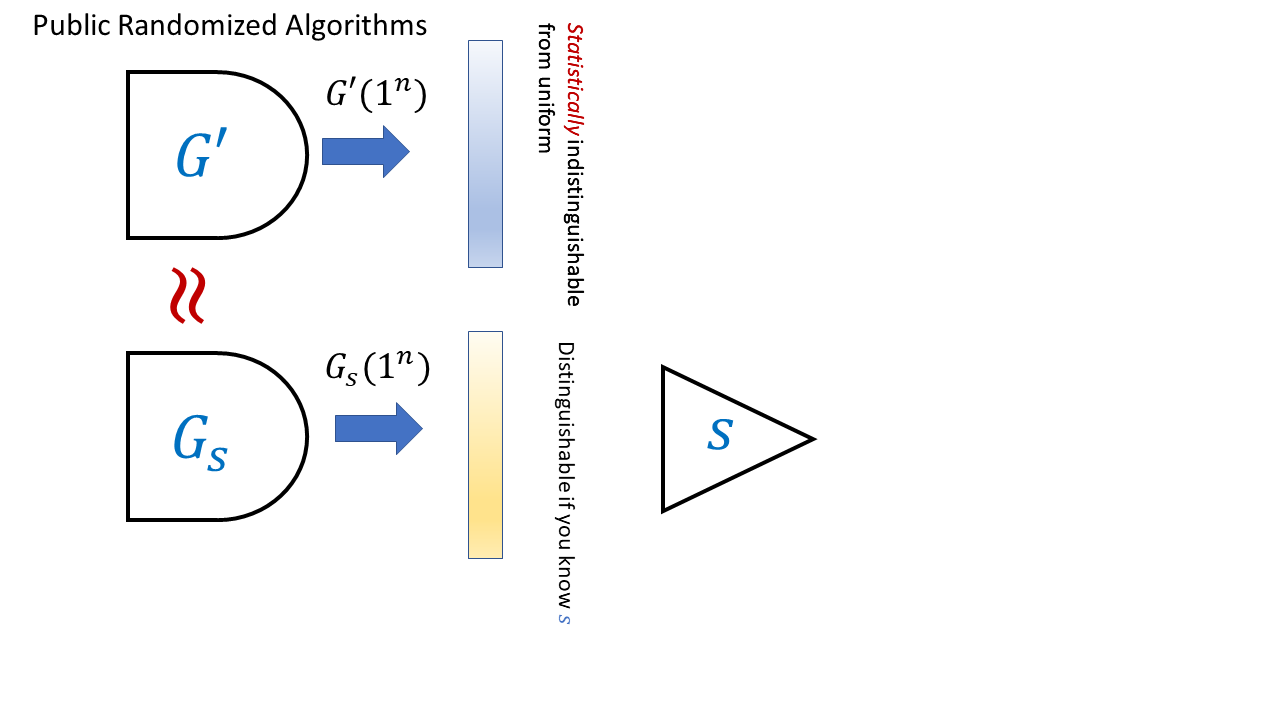
\includegraphics[width=\linewidth, height=1.5in, keepaspectratio]{../figure/trapdoorprg.png}
\caption{In a \emph{trapdoor generator}, we have two ways to generate
randomized algorithms. That is, we have some algorithms
\(\ensuremath{\mathit{GEN}}\) and \(\ensuremath{\mathit{GEN}}'\) such
that \(\ensuremath{\mathit{GEN}}\) outputs a pair \((G_s,s)\) and
\(\ensuremath{\mathit{GEN}}'\) outputs \(G'\) with \(G_s,G'\) being
themselves algorithms (e.g., randomized circuits). The conditions we
require are that \textbf{(1)} the descriptions of the circuits \(G_s\)
and \(G'\) (considering them as distributions over strings) are
computationally indistinguishable and \textbf{(2)} the distribution
\(G'(1^n)\) is \emph{statistically indistinguishable} from the uniform
distribution , \textbf{(3)} there is an efficient algorithm that given
the secret ``trapdoor'' \(s\) can distinguish the output of \(G_s\) from
the uniform distribution. In particular \textbf{(1)},\textbf{(2)}, and
\textbf{(3)} together imply that it is \emph{not} feasible to exract
\(s\) from the description of \(G_s\).}
\label{TDPgenfig}
\end{marginfigure}

Note that this trapdoor generator satisfies the following stronger
property: we can generate an alternative generator \(G'\) such that the
description of \(G'\) is indistinguishable from the description of
\(G_s\) but such that \(G'\) actually does produce (up to exponentially
small statistical error) the uniform distribution over \(\Z_q^n\). We
can define trapdoor generators formally as follows

\hypertarget{tdpgendef}{}
\begin{definition}[Trapdoor generators] \label[definition]{tdpgendef}

A \emph{trapdoor generator} is a pair of randomized algorithms
\(\ensuremath{\mathit{GEN}},\ensuremath{\mathit{GEN}}'\) that satisfy
the following:

\begin{itemize}
\item
  On input \(1^n\), \(\ensuremath{\mathit{GEN}}\) outputs a pair
  \((G_s,s)\) where \(G_s\) is a string describing a \emph{randomized}
  circuit that itself takes \(1^n\) as input and outputs a string of
  length \(t\) where \(t=t(n)\) is some polynomial.
\item
  On input \(1^n\), \(\ensuremath{\mathit{GEN}}'\) outputs \(G'\) where
  \(G'\) is a string describing a randomized circuit that itself takes
  \(1^n\) as input.
\item
  The distributions \(\ensuremath{\mathit{GEN}}(1^n)_1\) (i.e., the
  first output of \(\ensuremath{\mathit{GEN}}(1^n)\) and
  \(\ensuremath{\mathit{GEN}}'(1^n)\) are computationally
  indistinguishable
\item
  With probability \(1-negl(n)\) over the choice of \(G'\) output by
  \(\ensuremath{\mathit{GEN}}'\), the distribution \(G'(1^n)\) is
  \emph{statistically indistinguishable} (i.e., within \(negl(n)\) total
  variation distance) from \(U_t\).
\item
  There is an efficient algorithm \(T\) such that for every pair
  \((G_s,s)\) output by \(\ensuremath{\mathit{GEN}}\),
  \(\Pr[ T(s,G_s(1^n))=1] \geq 1- negl(n)\) (where this probability is
  over the internal randomness used by \(G_s\) on the input \(1^n\)) but
  \(\Pr[ T(s,U_t)=1] \leq 1/3\).\footnote{The choice of \(1/3\) is
    arbitrary, and can be amplified as needed.}
\end{itemize}

\end{definition}

\begin{pause} \label[pause]{16-This-is-not-an-easy-de}

This is not an easy definition to parse, but looking at \cref{TDPgenfig}
can help. Make sure you understand why \(\ensuremath{\mathit{LWEENC}}\)
gives rise to a trapdoor generator satisfying all the conditions of
\cref{tdpgendef}.

\end{pause}

\hypertarget{trapdoorgenreal}{}
\begin{remark}[Trapdoor generators in real life] \label[remark]{trapdoorgenreal}

In the above we use the notion of a ``trapdoor'' in the pseudorandom
generator as a mathematical abstraction, but generators with actual
trapdoors have arisen in practice. In 2007 the National Institute of
Standards (NIST) released standards for pseudorandom generators.
Pseudorandom generators are the quintessential private key primitive,
typically built out of hash functions, block ciphers, and such and so it
was surprising that NIST included in the list a pseudorandom generator
based on public key tools - the
\href{https://en.wikipedia.org/wiki/Dual_EC_DRBG}{Dual EC DRBG}
generator based on elliptic curve cryptography. This was already strange
but became even more worrying when Microsoft researchers Dan Shumow and
Niels Ferguson \href{http://rump2007.cr.yp.to/15-shumow.pdf}{showed}
that this generator \emph{could} have a trapdoor in the sense that it
contained some hardwired constants that if generated in a particular
way, there would be some information that (just like in \(G_s\) above)
allows to distinguish the generator from random (see here for a
\href{https://www.schneier.com/blog/archives/2007/11/the_strange_sto.html}{2007
blog post} on this issue). We learned more about this when leaks from
the Snowden document
\href{http://www.reuters.com/article/us-usa-security-rsa-idUSBRE9BJ1C220131220}{showed}
that the NSA secretly paid 10 million dollars to RSA to make this
generator the default option in their Bsafe software.

You'd think that this generator is long dead but it turns out to be the
``gift that keeps on giving''. In December of 2015, Juniper systems
\href{http://www.wired.com/2015/12/juniper-networks-hidden-backdoors-show-the-risk-of-government-backdoors/}{announced}
that they have discovered a malicious code in their system, dating back
to at least 2012 (possibly \href{https://goo.gl/X6pAXV}{2008}), that
would allow an attacker to surreptitiously decrypt all VPN traffic
through their firewalls. The issue is that Juniper has been using the
Dual EC DRBG and someone has managed to replace the constant they were
using with another one, one that they presumably knew the trapdoor for
(see
\href{https://rpw.sh/blog/2015/12/21/the-backdoored-backdoor/}{here} and
\href{http://blog.cryptographyengineering.com/2015/12/on-juniper-backdoor.html}{here}
for more; of course unless you know to check for this, it's very hard by
looking at the code to see that one arbitrary looking constant has been
replaced by another). Apparently, even though this is very surprising to
many people in law enforcement and government, inserting back doors into
cryptographic primitives might end up making them less secure.

\end{remark}

\section{From linear homomorphism to full
homomorphism}\label{16-From-linear-homomorphi}

Gentry's breakthrough had two components:

\begin{itemize}
\item
  First, he gave a scheme that is homomorphic with respect to arithmetic
  circuits (involving not just addition but also multiplications) of
  \emph{logarithmic depth}.
\item
  Second, he showed the amazing ``bootstrapping theorem'' that if a
  scheme is homomorphic enough to evaluate its own decryption circuit,
  then it can be turned into a \emph{fully homomorphic} encryption that
  can evaluate \emph{any} function.
\end{itemize}

Combining these two insights led to his fully homomorphic
encryption.\footnote{The story is a bit more complex than that.
  Frustratingly, the decryption circuit of Gentry's basic scheme was
  just a little bit too deep for the bootstrapping theorem to apply. A
  lesser man, such as yours truly, would at this point surmise that
  fully homomprphic encryption was just not meant to be, and perhaps
  take up knitting or playing bridge as an alternative hobby. However,
  Craig persevered and managed to come up with a way to ``squash'' the
  decryption circuit so it can fit the bootstrapping parameters. Follow
  up works, and in particular the paper of Brakerski and Vaikuntanathan,
  managed to get schemes with much better relation between the
  homomorphism depth and decryption circuit, and hence avoid the need
  for squashing and also improve the security assumptions.}

In this lecture we will focus on the second component - the
bootstrapping theorem. We will show a ``partially homomorphic
encryption'' (based on a later work of Gentry, Sahai and Waters) that
can fit that theorem in the next lecture.

\section{Bootstrapping: Fully Homomorphic ``escape
velocity''}\label{16-Bootstrapping-Fully-Ho}

\begin{marginfigure}
\centering
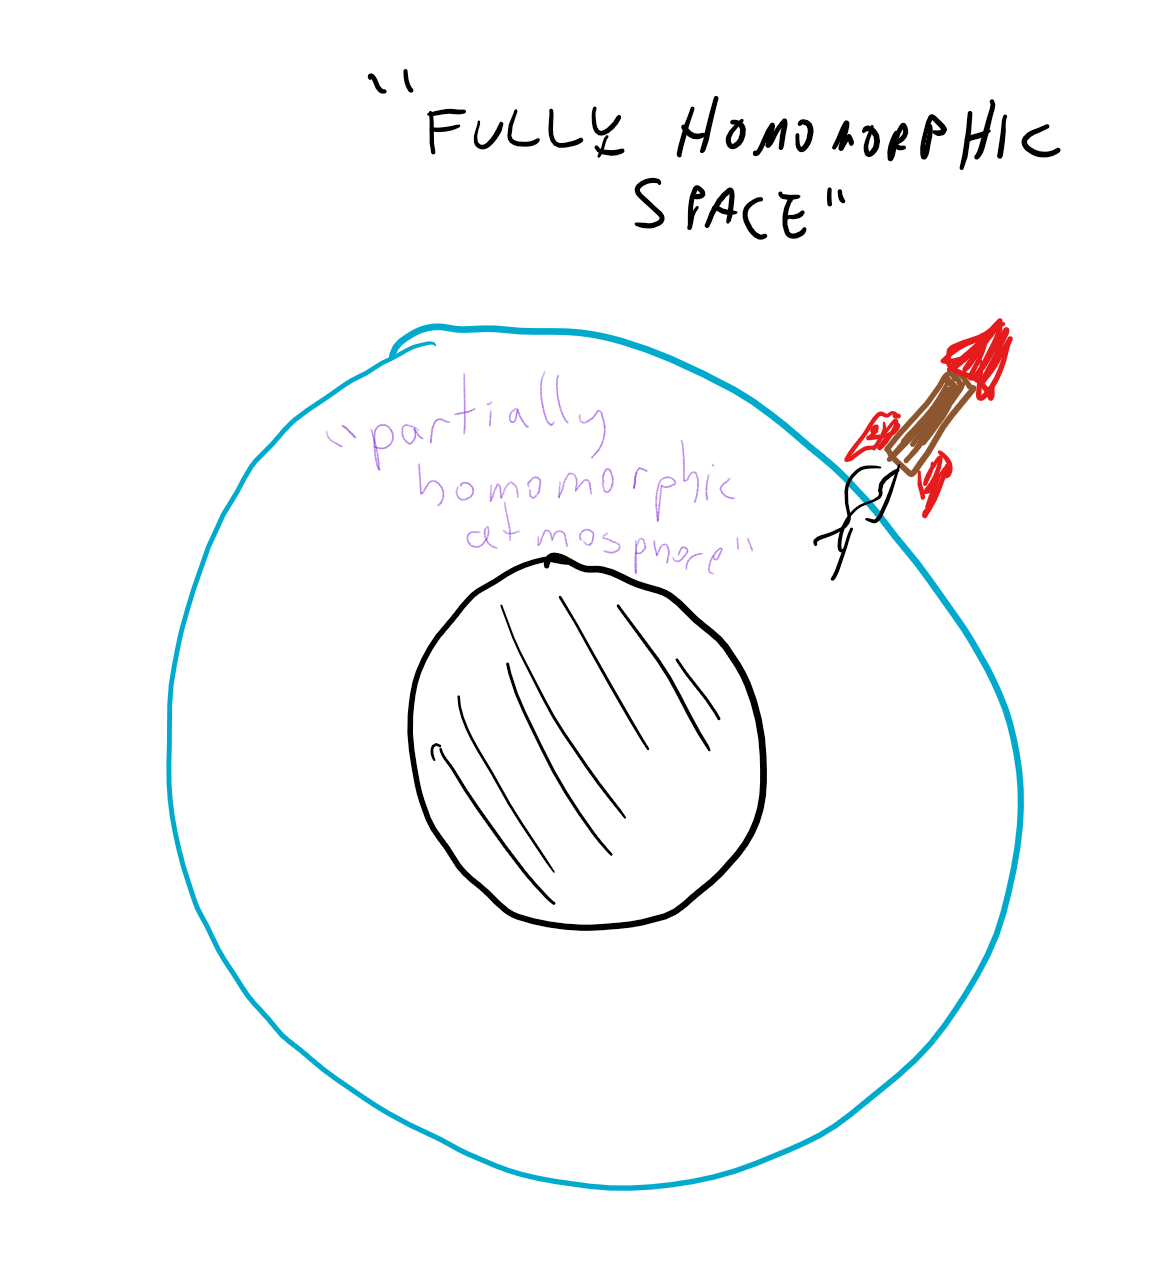
\includegraphics[width=\linewidth, height=1.5in, keepaspectratio]{../figure/fheescape.png}
\caption{The ``Bootstrapping Theorem'' shows that once a partially
homomorphic encryption scheme is homomorphic with respect to a rich
enough family of functions, and specifically a family that contains its
own decryption algorithm, then it can be converted to a fully
homomorphic encryption scheme that can be used to evaluate \emph{any}
function.}
\label{bootstrapfig}
\end{marginfigure}

The bootstrapping theorem is quite surprising. A priori you might expect
that given that a homomorphic encryption for linear functions was not
trivial to do, a homomorphic encryption for quadratics would be harder,
cubics even harder and so on and so forth. But it turns out that there
is some special degree \(t^*\) such that if we obtain homomorphic
encryption for degree \(t^*\) polynomials then we can obtain
\emph{fully} homomorphic encryption that works for \emph{all} functions.
(Specifically, if the decryption algorithm \(c \mapsto D_d(c)\) is a
degree \(t\) polynomial, then homomorphically evaluating polynomials of
degree \(t^*=2t\) will be sufficient.) That is, it turns out that once
an encryption scheme is strong enough to \emph{homomorphically evaluate
its own decryption algorithm} then we can use it to obtain a fully
homomorphic encryption by ``pulling itself up by its own bootstraps''.
One analogy is that at this point the encryption reaches ``escape
velocity'' and we can continue onwards evaluating gates in perpetuity.

We now show the bootstrapping theorem:

\hypertarget{bootstrapthm}{}
\begin{theorem}[Bootstrapping Theorem, Gentry 2009] \label[theorem]{bootstrapthm}

Suppose that \((G,E,D)\) is a CPA circular\footnote{You can ignore the
  condition of circular security in a first read - we will discuss it
  later.} secure partially homomorphic encryption scheme for the family
\(\mathcal{F}\) and suppose that for every pair of ciphertexts \(c,c'\)
the map \(d \mapsto D_d(c) \;\ensuremath{\mathit{NAND}}\; D_d(c')\) is
in \(\mathcal{F}\). Then \((G,E,D)\) can be turned a fully homomorphic
encryption scheme.

\end{theorem}

\subsection{Radioactive legos analogy}\label{16-Radioactive-legos-anal}

\begin{marginfigure}
\centering
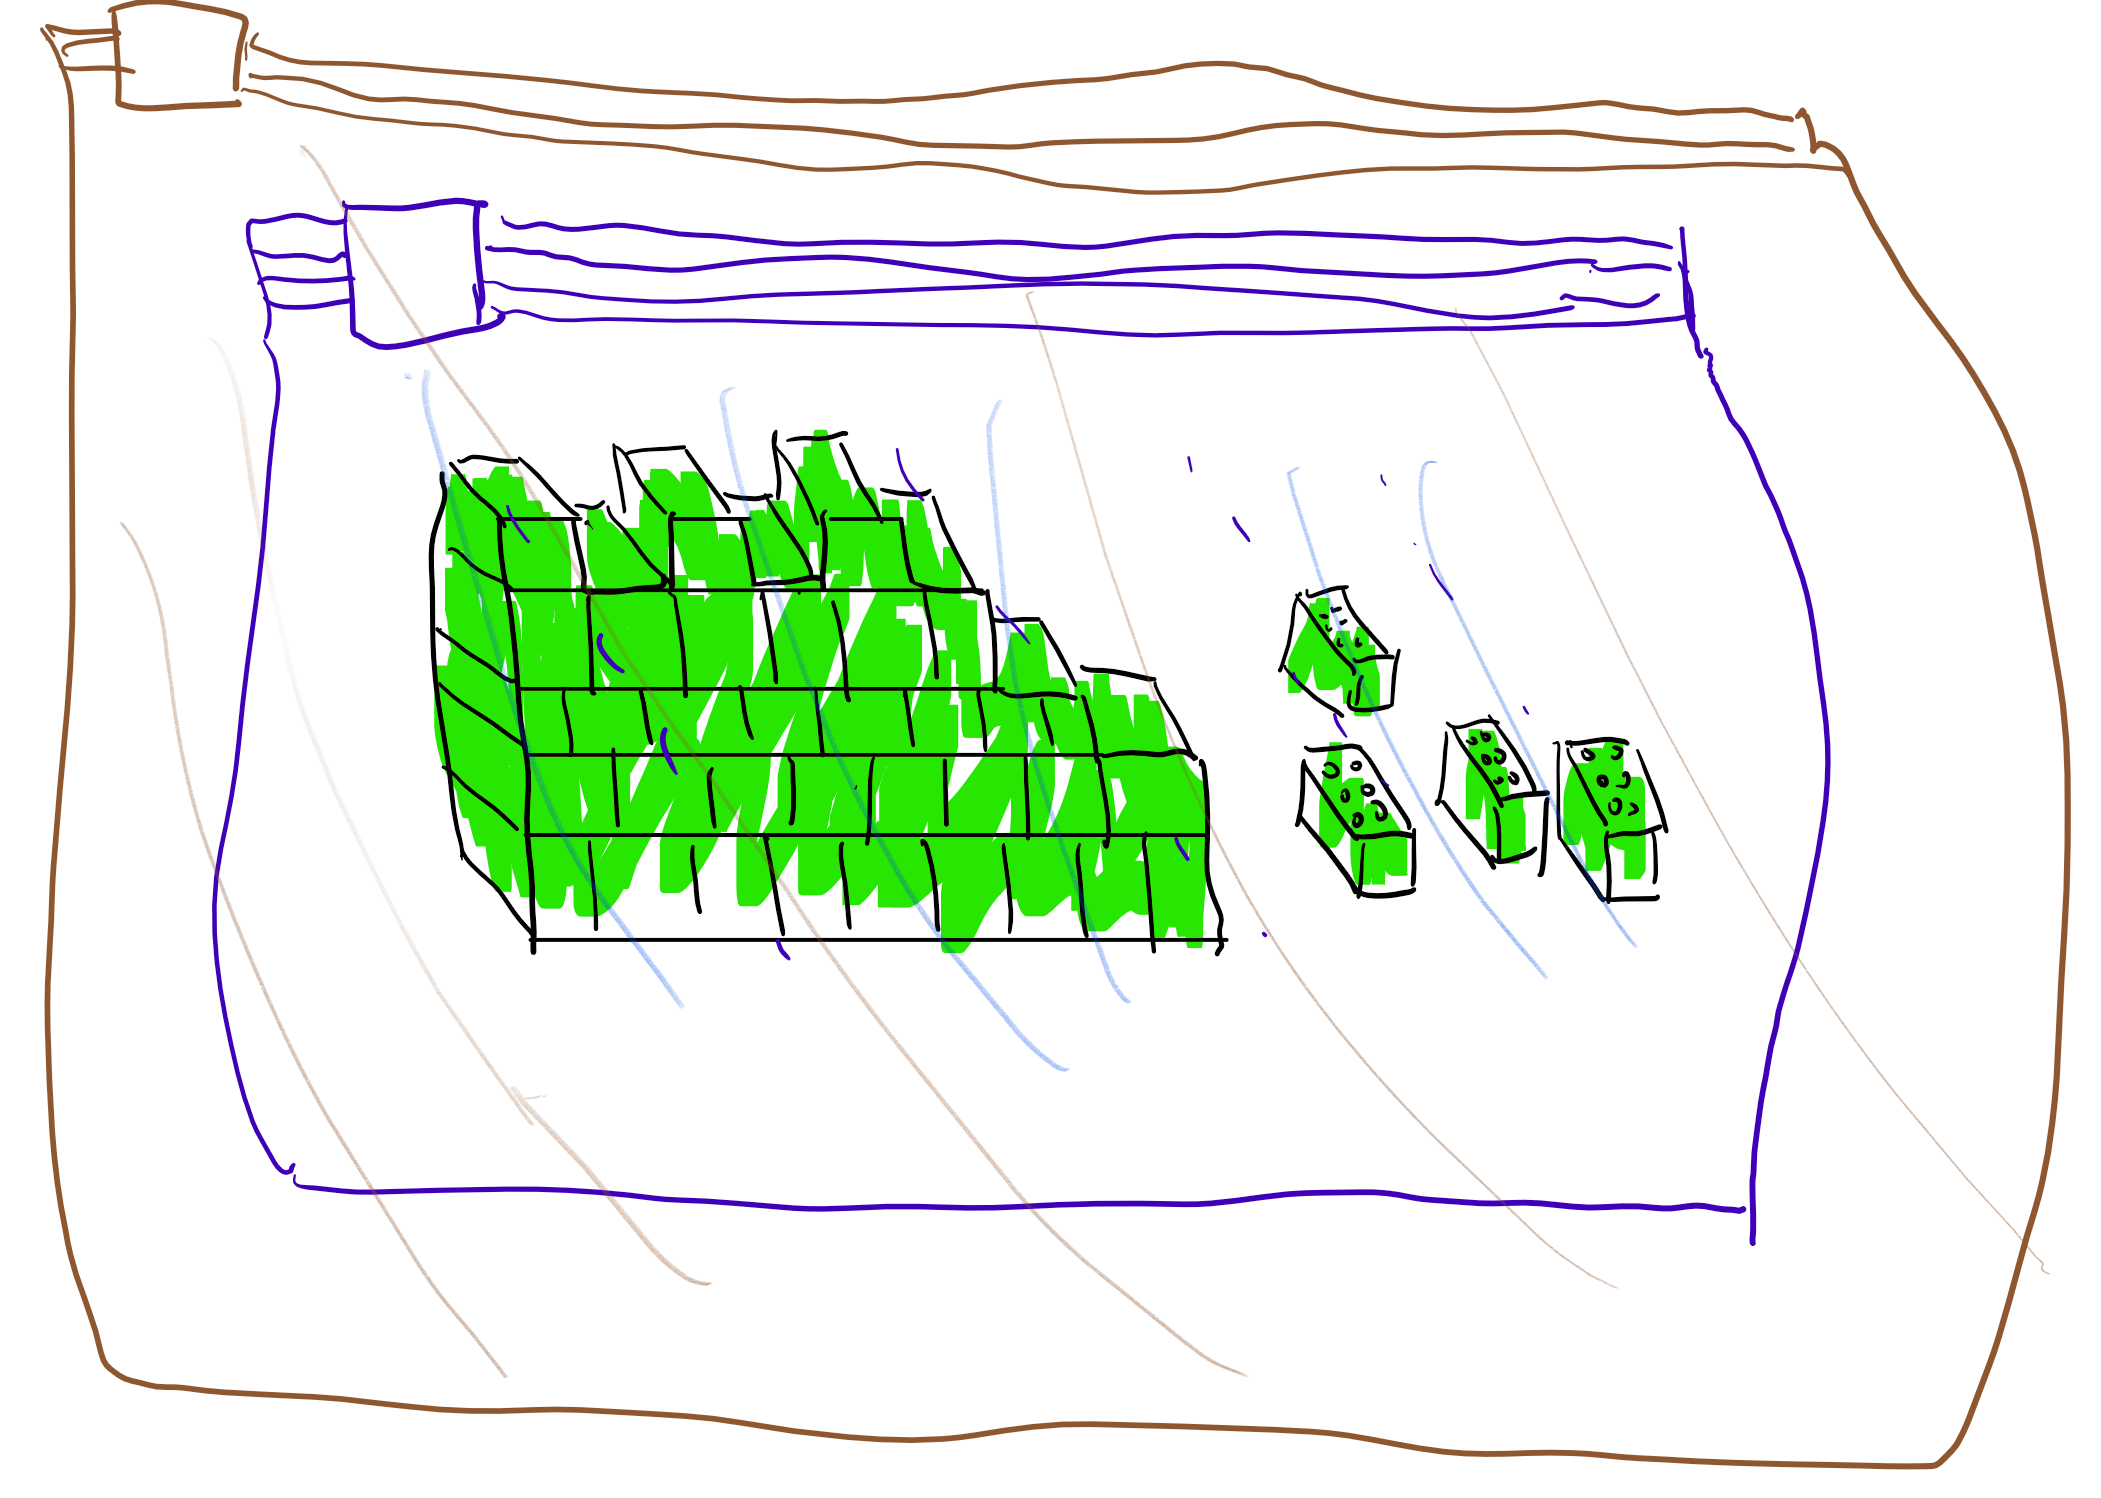
\includegraphics[width=\linewidth, height=1.5in, keepaspectratio]{../figure/fheziplocbag.png}
\caption{To build a castle from radioactive Lego bricks, which can be
kept safe in a special ziploc bag for 10 seconds, we can: 1) Place the
bricks in a bag, and place the bag inside an outer bag. 2) Manipulate
the inner bag through the outer bag to remove the bricks from it in 9
seconds, and spend 1 second putting one brick in place 3) Now the outer
bag has 9 seconds of life left, and we can put it inside a new bag and
repeat the process.}
\label{ziplocbagfig}
\end{marginfigure}

Here is one analogy for bootstrapping, inspired by Gentry's
\href{https://crypto.stanford.edu/craig/easy-fhe.pdf}{survey}. Suppose
that you need to construct some complicated object from a highly toxic
material (see \cref{ziplocbagfig}). You are given a supply of sealed
bags that are flexible enough so you can manipulate the object from
outside the bag. However, each bag can only hold for \(10\) seconds of
such manipulations before it leaks. The idea is that if you can open one
bag inside another within \(9\) seconds then you can perform the
manipulations for arbitrary length. That is, if the object is in the
\(i^{th}\) bag then you put this bag inside the \(i+1^{st}\) bag, spend
\(9\) seconds on opening the \(i^{th}\) bag inside the \(i+1^{st}\) bag
and then spend another second of whatever manipulations you wanted to
perform. We then continue this process by putting the \(i+1^{st}\) bag
inside the \(i+2^{nd}\) bag and so on and so forth.

\subsection{Proving the bootstrapping
theorem}\label{16-Proving-the-bootstrapp}

We now turn to the formal proof of \cref{bootstrapthm}

\begin{proof} \label[proof]{16-The-idea-behind-the-pr}

The idea behind the proof is simple but ingenious. Recall that the NAND
gate \(b,b' \mapsto \neg(b \wedge b')\) is a universal gate that allows
us to compute any function \(f:\{0,1\}^n\rightarrow\{0,1\}\) that can be
efficiently computed. Thus, to obtain a fully homomorphic encryption it
suffices to obtain a function \(\ensuremath{\mathit{NANDEVAL}}\) such
that
\(D_d(\ensuremath{\mathit{NANDEVAL}}(c,c'))=D_d(c) \;\ensuremath{\mathit{NAND}}\; D_d(c')\).
(Note that this is stronger than the typical notion of homomorphic
evaluation since we require that \(\ensuremath{\mathit{NANDEVAL}}\)
outputs an encryption of \(b \;\ensuremath{\mathit{NAND}}\; b'\) when
given \emph{any} pair of ciphertexts that decrypt to \(b\) and \(b'\)
respectively, regardless whether these ciphertexts were produced by the
encryption algorithm or by some other method, including the
\(\ensuremath{\mathit{NANDEVAL}}\) procedure itself.)

Thus to prove the theorem, we need to modify \((G,E,D)\) into an
encryption scheme supporting the \(\ensuremath{\mathit{NANDEVAL}}\)
operation. Our new scheme will use the same encryption algorithms \(E\)
and \(D\) but the following modification \(G'\) of the key generation
algorithm: after running \((d,e)=G(1^n)\), we will append to the public
key an encryption \(c^* = E_e(d)\) of the secret key. We have now
defined the key generation, encryption and decryption. CPA security
follows from the security of the original scheme, where by circular
security we refer exactly to the condition that the scheme is secure
even if the adversary gets a single encryption of the public
key.\footnote{Without this assumption we can still obtained a form of
  FHE known as a \emph{leveled} FHE where the size of the public key
  grows with the
  \href{https://en.wikipedia.org/wiki/Circuit_complexity}{depth} of the
  circuit to be evaluated. We can do this by having \(\ell\) public keys
  where \(\ell\) is the depth we want to evaluate, and encrypt the
  private key of the \(i^{th}\) key with the \(i+1^{st}\) public key.
  However, since circular security seems quite likely to hold, we ignore
  this extra complication in the rest of the discussion.} This latter
condition is not known to be implied by standard CPA security but as far
as we know is satisfied by all natural public key encryptions, including
the LWE-based ones we will plug into this theorem later on.

So, now all that is left is to define the
\(\ensuremath{\mathit{NANDEVAL}}\) operation. On input two ciphertexts
\(c\) and \(c'\), we will construct the function
\(f_{c,c'}:\{0,1\}^n\rightarrow\{0,1\}\) (where \(n\) is the length of
the secret key) such that
\(f_{c,c'}(d)=D_d(c) \;\ensuremath{\mathit{NAND}}\; D_d(c')\). It would
be useful to pause at this point and make sure you understand what are
the inputs to \(f_{c,c'}\), what are ``hardwired constants'' and what is
its output. The ciphertexts \(c\) and \(c'\) are simply treated as fixed
strings and are \emph{not} part of the input to \(f_{c,c'}\). Rather
\(f_{c,c'}\) is a function (depending on the strings \(c,c'\)) that maps
the secret key into a bit. When running
\(\ensuremath{\mathit{NANDEVAL}}\) we of course do not know the secret
key \(d\), but we can still design a circuit that computes this function
\(f_{c,c'}\). Now \(\ensuremath{\mathit{NANDEVAL}}(c,c')\) will simply
be defined as \(\ensuremath{\mathit{EVAL}}(f_{c,c'},c^*)\). Since
\(c^* = E_e(d)\), we get that
\begin{equation*}
D_d(\ensuremath{\mathit{NANDEVAL}}(c,c'))= D_d(\ensuremath{\mathit{EVAL}}(f_{c,c'},c^*))=f_{c,c'}(d) =D_d(c) \;\ensuremath{\mathit{NAND}}\; D_d(c') \;.
\end{equation*}
Thus indeed we map \emph{any} pair of ciphertexts \(c,c'\) that decrypt
to \(b,b'\) into a ciphertext \(c''\) that decrypts to
\(b \;\ensuremath{\mathit{NAND}}\; b'\). This is all that we needed to
prove.

\end{proof}

\begin{pause} \label[pause]{16-Dont-let-the-short-pro}

Don't let the short proof fool you. This theorem is quite deep and
subtle, and requires some reading and re-reading to truly ``get'' it.

\end{pause}
